\begin{figure*}[t]
\centering
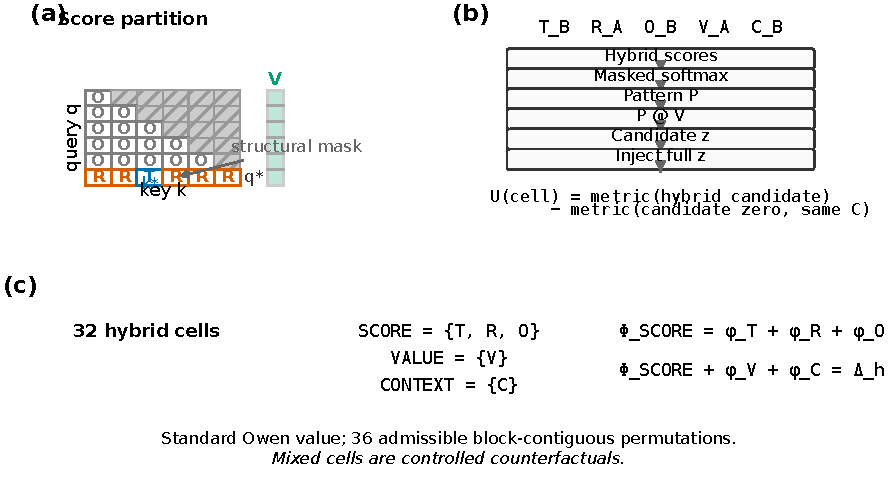
\includegraphics[width=\textwidth]{figures/Fig2.pdf}
\caption{\textbf{FALI constructs a 32-cell counterfactual intervention game for the selected attention head.}
(a) Structurally valid pre-softmax scores are partitioned into the prespecified task-target coordinate(s) $T$, rival scores $R$ in the same task-relevant query row, and all other valid scores $O$; masked coordinates are not players.
(b) Each hybrid cell selects $T,R,O,V,$ and $C$ from the intact or perturbed endpoint, reconstructs the candidate attention pattern and head output, and defines utility relative to a candidate-zero run in the same surrounding context $C$.
(c) All $2^5=32$ hybrid states are evaluated. Standard Owen attribution under $\mathrm{SCORE}=\{T,R,O\}$, $\mathrm{VALUE}=\{V\}$, and $\mathrm{CONTEXT}=\{C\}$ allocates the endpoint change over 36 block-contiguous admissible permutations, satisfying $\sum_i\phi_i=\Delta_h$ and $\Phi_{\mathrm{SCORE}}=\phi_T+\phi_R+\phi_O$.
The mixed cells are controlled counterfactual states, not claims that the model naturally implements five independent causal pathways.}
\label{fig:fali-game}
\end{figure*}
